% 第三章 研究設計與預先登錄（對應英文稿 Section 3, en/front.tex）
\chapter{研究設計與預先登錄}
\label{zh:sec:design}

\section{三項研究概覽}
\label{zh:sec:design_overview}

圖~\ref{zh:fig:research_design} 與表~\ref{zh:tab:front_overview} 彙整了本研究的設計。RQ1 由研究一以及研究二的領域層次與格層次分析處理；RQ2 由研究二的公司層次分析處理；RQ3 與 RQ4 則由第~\ref{zh:sec:mlp}~節處理，該節亦說明研究三——一項計畫，而非結果的來源。系統性文獻回顧與 R1（第~\ref{zh:sec:review}~節）則探討此一推論在本專案之外的普遍程度。在三條資料線中，僅有專利提供了可用的流動（flow）資料（第~\ref{zh:sec:theory_cooccurrence}~節與第~\ref{zh:sec:design_sources}~節），且三個層次的專利分析共用同一資料來源，因此彼此並不獨立。

\begin{figure}[tbp]
\centering
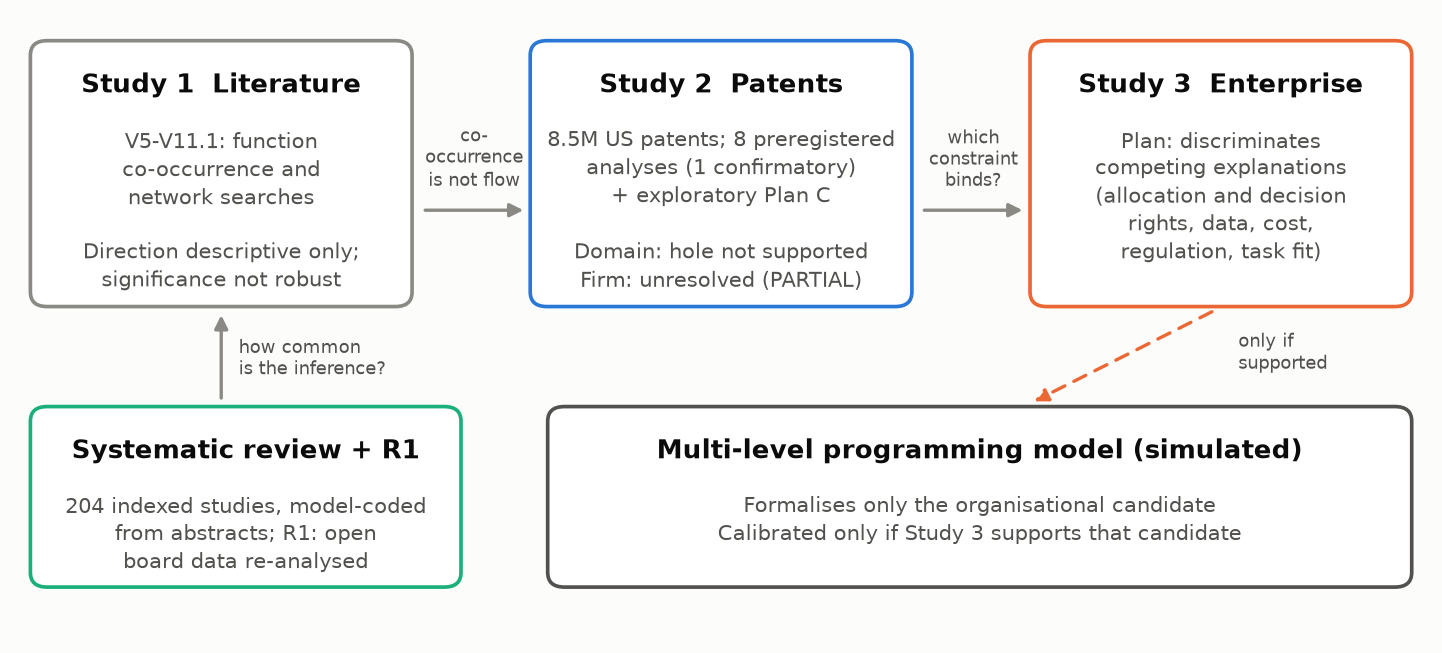
\includegraphics[width=\linewidth]{fig_research_design.png}
\caption[研究設計]{研究設計。研究一（文獻，V5--V11.1）顯示共現（co-occurrence）不等於流動；其方向僅屬描述性，且其顯著性並不穩健。研究二（美國專利；六項預先登錄〔preregistered〕的分析，其中一項為驗證性〔計畫 1〕、五項受資料啟發〔計畫 2--6，其中計畫 6 未通過其合格檢查〕，另加探索性的計畫 C；AI = CPC G06N；決策 = CPC G06Q10/04 與 G06Q10/06，而非整個 G06Q10）處理 RQ1 與 RQ2；圖中的概數對應 8,512,829 件發明專利（utility patents）。在領域層次，知識流動中的結構洞（structural hole）未獲支持（\texttt{HOLE\_\allowbreak NOT\_\allowbreak SUPPORTED}），但這並未證明結構洞不存在。在公司層次，此一問題仍未解決（判定為 \texttt{PARTIAL}）：在專利組合構成之外，仍存在顯著的專門型公司分隔，而混合型公司是否為其中介者（broker），無法以現有的虛無模型（null model）判定。因此，研究二未能釐清何種限制條件具有約束力。系統性文獻回顧（204 篇已索引研究，以模型依摘要層次編碼）與對公開董事會資料的 R1 重新分析，探討此一推論的普遍程度。研究三是一項尚無結果的規劃中企業研究，旨在區辨五種競爭解釋（competing explanations）。三層規劃模型（第 1 層：資源分配〔resource allocation〕；第 2 層：AI 架構與治理；第 3 層：人機配置）僅將組織層面的候選解釋形式化；其參數為模擬值，且僅在研究三支持該候選解釋時才會加以校準（虛線箭頭）。}
\label{zh:fig:research_design}
\end{figure}

\begin{table}[tbp]
\centering
\footnotesize
\setlength{\tabcolsep}{4pt}
\caption[研究與資料線概覽]{研究與資料線概覽。來源等級（provenance grade）的定義見第~\ref{zh:sec:design_prereg}~節：DIRECT；HIST.\ = HISTORICAL；USER = USER\_\allowbreak REPORTED；SIM.\ = SIMULATED。}
\label{zh:tab:front_overview}
\begin{tabular}{@{}p{0.16\linewidth}p{0.25\linewidth}p{0.16\linewidth}p{0.25\linewidth}p{0.09\linewidth}@{}}
\toprule
研究／資料線（狀態） & 資料 & 關係類型 & 主要檢定 & 等級 \tabularnewline
\midrule
\raggedright 研究一：功能矩陣（已完成） &
\raggedright 2,118 份來源文件；10 $\times$ 12 矩陣中 2,180 條文件層次的邊 &
\raggedright 共現（二模） &
\raggedright 四項虛無模型檢定並以 BH 偽發現率（FDR）校正；誤分類界限與模擬 &
\raggedright DIRECT \tabularnewline
\addlinespace
\raggedright 研究一：網路資料線 V6--V11.1（已完成） &
\raggedright 引用、共同著作與高階網路 &
\raggedright 引用篩檢與投影 &
\raggedright 搜尋 Burt 意義下的中介者；外部審查 &
\raggedright HIST.\ / USER \tabularnewline
\addlinespace
\raggedright 外部資料篩檢（已完成） &
\raggedright 六個公開來源（CORDIS H2020、GLEIF、OpenAlex、OCDS、SEC、PyPSA） &
\raggedright 隸屬、所有權、實體拓樸 &
\raggedright 獨立關係關卡與驗證關卡 &
\raggedright DIRECT \tabularnewline
\addlinespace
\raggedright 研究二：專利（已完成） &
\raggedright 8,512,829 件美國發明專利；AI = G06N；DEC = G06Q10/04 + G06Q10/06 &
\raggedright 有向申請人引用 &
\raggedright 六項預先登錄分析（計畫 1 為驗證性；計畫 2--6 受資料啟發；計畫 6 為 \texttt{INVALID\_\allowbreak NULL}）：總體檢定、CPC 矩陣、複製分析套組、兩個公司虛無模型、構念效度檢查；探索性的計畫 C &
\raggedright DIRECT \tabularnewline
\addlinespace
\raggedright 系統性文獻回顧與 R1（已完成） &
\raggedright 204 篇已索引研究（OpenAlex），由大型語言模型代理依摘要編碼；挪威董事會檔案（R1） &
\raggedright 依編碼：共現或隸屬；R1：二模隸屬 &
\raggedright 失效模式 F1--F4 與驗證 V 的盛行率；R1：保留隸屬結構的虛無模型 &
\raggedright DIRECT \tabularnewline
\addlinespace
\raggedright MLP 原型（示例） &
\raggedright 3 個流程；參數組 C／F／D；預算 3／5／7 &
\raggedright 無（模擬參數） &
\raggedright 精確逆向歸納 &
\raggedright SIM. \tabularnewline
\addlinespace
\raggedright 研究三：企業（計畫） &
\raggedright 一家或多家製造業公司的決策流程 &
\raggedright 規劃中的企業資料 &
\raggedright 以預先登錄的判定規則區辨競爭解釋 &
\raggedright -- \tabularnewline
\bottomrule
\end{tabular}
\end{table}

\section{選擇具流動效度的資料來源}
\label{zh:sec:design_sources}

在轉向專利之前，本研究以兩道關卡篩檢了六個公開的關係資料來源：獨立關係關卡與驗證關卡。CORDIS H2020（35,389 個專案；179,063 筆組織參與紀錄）產生的是共同成員關係，而非流動。在包含 49 次重複的保留度數二分交換虛無模型下，其 5 個可檢定的低限制度候選者之 $p$ = .41--.86，BH $q \geq .80$ \citep{benjamini1995controlling}；達顯著者為 0 個。GLEIF Level-2（663,449 筆關係紀錄，其中 481,247 筆為有效狀態）記錄的是法律上的合併（consolidation）關係。OpenAlex 回傳 8 筆著作，OCDS 回傳 0 條可驗證的採購者—供應者邊，而 PyPSA（8,786 個匯流排）描述的是實體電網。SEC 申報文件並未擷取，因為其存取需要真實的聯絡用 User-Agent。沒有任何來源同時通過兩道關卡：共同成員關係、所有權與實體拓樸皆非資訊流動。附錄表~\ref{zh:tab:app_sources} 報告完整的篩檢結果。

專利符合第~\ref{zh:sec:theory_holes}~節所述的要求。引用是有向流動 \citep{jaffe1993geographic}，CPC 分類是由審查員而非分析者指派的標籤，且資料涵蓋美國核准專利的母體，而非樣本。

\section{預先登錄紀錄與來源等級}
\label{zh:sec:design_prereg}

研究二以六項計畫進行預先登錄（preregistration）：計畫 1為總體領域檢定；計畫 2為在 CPC 格矩陣上進行的 V9 檢定組合；計畫 3為包含模組 P1--P10 的完整複製分析套組；計畫 4為保留專利組合的公司虛無模型（portfolio-preserving null）；計畫 5為構念效度（construct validity）檢查，係在計畫 1 的判定已知之後才擬定的後續分析（受資料啟發）；計畫 6為另依度數分層的公司虛無模型。探索性的計畫 C 則描述跨領域引用發生在哪裡。系統性文獻回顧的計畫書與 R1 重新分析計畫則另行凍結（附錄~\ref{zh:app:review}）。上述各項皆為專案儲存庫中的提交（commit）（為審查之故隱去識別碼；列於附錄~\ref{zh:app:prereg} 表~\ref{zh:tab:app_prereg} 與表~\ref{zh:tab:app_prereg_b}）。預先登錄的用意，是在觀察到結果之前固定分析計畫，以區分驗證性分析與探索性分析 \citep{nosek2018preregistration}。以下三項限定，界定了本研究的計畫在多大程度上符合此一標準。

第一，這些計畫是專案自有儲存庫中自行加註時間戳記的 git 提交，而非向第三方（例如開放科學架構〔Open Science Framework, OSF〕）所做的登錄；其時間戳記受作者控制，無法獨立驗證。第二，僅有計畫 1早於所有專利結果：它在下載任何專利資料之前即已凍結。計畫 2至計畫 6皆是在先前結果已知之後撰寫的，因此其研究問題受到資料的影響；只有其定義、虛無模型、判定規則、門檻、敏感度分析與停止規則（stop rule）是在計算之前固定的。計畫 4的動機來自計畫 3（模組 P5）的公司網路結果，並在計算其虛無模型重複樣本之前凍結；該虛無模型並非獨立於該結果而選定。第三，M06-P（專利適用之保留文件結構虛無模型）並不屬於計畫 2：它是在預先登錄的交換虛無模型失效之後，才於計畫 3（模組 P1）中凍結的（修訂 B1，第~\ref{zh:sec:study2_cells}~節）。因此，本研究將計畫 1視為驗證性的，而將計畫 2至計畫 6視為受資料影響的後續分析，其規則——而非其研究問題——是事先固定的。

偏離原計畫之處，以註明日期且不更動凍結文本的修訂（amendment）加以記錄（附錄表~\ref{zh:tab:app_amend}）。修訂 A1 在計算任何引用結果之前更正了一個 CPC 標籤的拼寫，並未改變設計中的任何內容。修訂 A2 記錄僅含申請人引用的設定實際上涵蓋 2013--2025 年的施引年份，並記錄計畫 1的 H3（一個以領域層次存在結構洞為條件的受讓人中介問題）因 H1 未獲支持而未執行；其後的公司分析（計畫 3，P5）係另行預先登錄，探討的是 RQ2，而 RQ2 並不以領域層次存在結構洞為前提。修訂 B1 記錄，預先登錄的格「核心」（core）——即在主要檢定、精確檢定與保留文件結構檢定（M06；調整後核心則為 M06-P）中皆為 $q \le .05$ 且方向相同，並且原始紀錄檢定亦為 $q \le .05$ 且方向相同的格；見第~\ref{zh:sec:study1_corpus}~節——在建構上即為空集合，因此以其餘三項檢定為依據的格結果屬於探索性。修訂 C1 在計畫 5 的初步結果已知之後、但在新增設定計算之前，為計畫 5 加入兩項更嚴格的構念設定。計畫 6 先以 2 次重複進行冒煙測試（smoke test），並將其檢定結果密封不讀；該測試已顯示合格檢查未通過，之後才進行完整執行。在系統性文獻回顧中，修訂 S1 在編碼之前擴大了裁決範圍；修訂 R1-A1 則在下載任何資料之前，加入原文章自身所用的快照。計畫 C 是一項探索性描述，說明跨領域引用發生在哪裡；它在計算之前即已凍結，但不檢定任何假設。研究一的資料效度再分析屬事後（post hoc）分析。

本研究中的每一個數字皆源自一份已記錄的結果檔，並具有三種來源等級（provenance grade）之一。DIRECT 數字係由凍結檔案重新計算或解析而得。HISTORICAL 數字報告於較早的專案紀錄中，其原始檔案已無法取得以重新驗證。USER\_\allowbreak REPORTED 數字則由研究者依據本地保存的檔案所報告。凡等級攸關之處，本研究皆予以註明；V6--V11.1 的網路結果屬 HISTORICAL 或 USER\_\allowbreak REPORTED，而 MLP 的輸出則為 SIMULATED。

\section{主張邊界}
\label{zh:sec:design_boundaries}

以下邊界規範本研究中的每一項主張：
\begin{enumerate}
\item[(i)] 在任何層次上，皆不主張已證實的結構洞。
\item[(ii)] 16 個 V9 偏低格，以及在 CPC 矩陣兩部分中皆偏低的 5 個專利格，均不稱為研究缺口。16 個 V9 格已撤回，不再作為 MLP 模型的依據。
\item[(iii)] 不主張任何因果效果。
\item[(iv)] MLP 的輸出為模擬結果，不反映任何真實公司。
\item[(v)] 「瓶頸在於組織」僅是數個候選解釋之一，並且是研究三的一項假說，而非研究結果。
\item[(vi)] 模型之間的一致性是可重現性的證據，而非人工信度的證據。
\item[(vii)] HISTORICAL 與 USER\_\allowbreak REPORTED 數據（V6--V11.1）皆如實標示。
\item[(viii)] 研究一偏低格的方向是一項描述，可能反映非隨機的編碼假象；它並非已證實的發現。
\end{enumerate}
全文中，「偏低」（depleted）與「偏高」（enriched）是相對於虛無模型對某一格所做的統計描述。它們本身並不構成領域之間存在分隔的證據。
